%% beamer packages
% other themes: AnnArbor, Antibes, Bergen, Berkeley, Berlin, Boadilla, boxes,
% CambridgeUS, Darmstadt, Dresden, Frankfurt, Goettingen, Hannover, Ilmenau,
%JuanLesPins, Luebeck, Madrid, Malmoe, Marburg, Montpellier, PaloAlto,
%Pittsburgh, Rochester, Singapore, Szeged, Warsaw
% other colors: albatross, beaver, crane, default, dolphin, dove, fly, lily,
%orchid, rose, seagull, seahorse, sidebartab, structure, whale, wolverine,
%beetle

%\documentclass[xcolor=dvipsnames]{beamer}
\documentclass[table,dvipsnames]{beamer}
\usepackage{beamerthemesplit}
\usepackage{bm,amsmath,marvosym}
\usepackage{listings,color}%xcolor
\usepackage[ngerman]{babel}
\usepackage{natbib}
\usepackage[utf8]{inputenc}
\usepackage{minted}
\definecolor{shadecolor}{rgb}{.9, .9, .9}
\definecolor{darkblue}{rgb}{0.0,0.0,0.5}
\definecolor{myorange}{cmyk}{0,0.7,1,0}
%\definecolor{mypurple}{cmyk}{0.5,1.0,0,0.2}
\definecolor{mypurple}{cmyk}{0.3, 0.9, 0.0, 0.2}

% make a checkmark
\usepackage{tikz}
\def\checkmark{\tikz\fill[scale=0.4](0,.35) -- (.25,0) -- (1,.7) -- (.25,.15) -- cycle;}

% math stuff
\newcommand{\argmin}{\operatornamewithlimits{argmin}}

\hypersetup{colorlinks = true, linkcolor=darkblue, citecolor=darkblue,urlcolor=darkblue}
\hypersetup{pdfauthor={E. Wellinger}, pdftitle={Random Forests}}

\newcommand{\rd}{\textcolor{red}}
\newcommand{\grn}{\textcolor{green}}
\newcommand{\keywd}{\textcolor{myorange}}
\newcommand{\highlt}{\textcolor{darkblue}}
\newcommand{\norm}[1]{\left\lVert#1\right\rVert}
\def\ci{\perp\!\!\!\perp}
% set beamer theme and color
\usetheme{Frankfurt}
%\usetheme{Berkeley}
\usecolortheme{seahorse}
% \usecolortheme{seagull}
%\setbeamertemplate{blocks}[rounded][shadow=true]

\title[Random Forests]{Random Forests}
\author[EKW]{Erich Wellinger}
\institute{Galvanize, Inc}
\date[\today]{Last updated: \today}

%%%%%%%%%%%%%%%%%%%%%%%%%%%%%%%%%%%%%%%%%%%%%%%%%%%%%%%%%%%%%%%%%%%%%%%%%%%%%%%
\begin{document}
\frame{\titlepage}
%%%%%%%%%%%%%%%%%%%%%%%%%%%%%%%%%%%%%%%%%%%%%%%%%%%%%%%%%%%%%%%%%%%%%%%%%%%%%%%
\frame{
\footnotesize
\tableofcontents
\normalsize
}

%%%%%%%%%%%%%%%%%%%%%%%%%%%%%%%%%%%%%%%%%%%%%%%%%%%%%%%%%%%%%%%%%%%%%%%%%%%%%%%

\begin{frame}
\frametitle{Objectives}
\scriptsize

Morning Objectives:
\begin{block}{}
\begin{itemize}
    \item Review
    \item Explain the construction of a \keywd{Random Forest} (classification or regression) algorithm
    \item Explain the relationship and difference between \keywd{bagging} and random forests
    \item Explain why random forests often perform better than a single decision tree
\end{itemize}
\end{block}

Afternoon Objectives:
\begin{block}{}
\begin{itemize}
    \item Explain how to get \keywd{feature importances} from a random forest and what those importances mean
    \item Explain \keywd{OOB error} is calculated and what it is an estimate of
\end{itemize}
\end{block}

\end{frame}

%%%%%%%%%%%%%%%%%%%%%%%%%%%%%%%%%%%%%%%%%%%%%%%%%%%%%%%%%%%%%%%%%%%%%%%%%%%%%%%

\begin{frame}
\frametitle{Agenda}
\scriptsize
Morning Agenda:

\begin{block}{}
\begin{itemize}
    \item Review decision trees
    \item Discuss ensemble methods
    \item Discuss \keywd{Bagging} (bootstrap aggregation)
    \item Discuss \keywd{Random Forests}
\end{itemize}
\end{block}

Afternoon Agenda:

\begin{block}{}
\begin{itemize}
    \item Discuss \keywd{Feature Importance}
    \item Discuss \keywd{Out-Of-Bag Error}
\end{itemize}
\end{block}
\end{frame}


%%%%%%%%%%%%%%%%%%%%%%%%%%%%%%%%%%%%%%%%%%%%%%%%%%%%%%%%%%%%%%%%%%%%%%%%%%%%%%%
\section{Review}
\subsection{}
%%%%%%%%%%%%%%%%%%%%%%%%%%%%%%%%%%%%%%%%%%%%%%%%%%%%%%%%%%%%%%%%%%%%%%%%%%%%%%%

\begin{frame}
\frametitle{Classification Trees}
Training:
\begin{itemize}
    \item Iteratively divide the nodes into subnodes such that (entropy/gini impurity) is minimized
    \item Various stopping conditions like a depth limit
    \item Prune trees by merging nodes
\end{itemize}

Inference:
\begin{itemize}
    \item Take the most common class in the leaf node
\end{itemize}
\end{frame}

%%%%%%%%%%%%%%%%%%%%%%%%%%%%%%%%%%%%%%%%%%%%%%%%%%%%%%%%%%%%%%%%%%%%%%%%%%%%%%%

\begin{frame}
\frametitle{Classification Trees}
\begin{center}
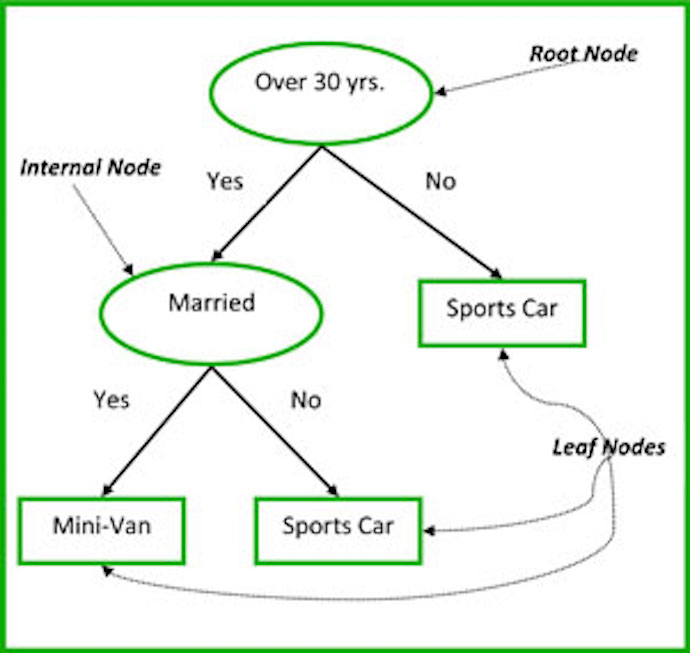
\includegraphics[scale=0.25]{imgs/decision_tree.png}
\end{center}
\end{frame}

%%%%%%%%%%%%%%%%%%%%%%%%%%%%%%%%%%%%%%%%%%%%%%%%%%%%%%%%%%%%%%%%%%%%%%%%%%%%%%%

\begin{frame}
\frametitle{Regression Trees}
Similar to Classification Trees but...
\begin{itemize}
    \item Instead of predicting a class label we're trying to predict a number
    \item We minimize \textit{total squared error} instead of entropy or impurity
    \begin{equation}
        \sum_{j=1}^J \sum_{i \in R_j} (y_i - \hat{y}_{R_j})^2
    \end{equation}
    \item Our prediction for any point that ends at that leaf node is simply the mean of the leaf node
\end{itemize}
\end{frame}

%%%%%%%%%%%%%%%%%%%%%%%%%%%%%%%%%%%%%%%%%%%%%%%%%%%%%%%%%%%%%%%%%%%%%%%%%%%%%%%

\begin{frame}
\frametitle{Regression Trees}
\begin{columns}[T]
\begin{column}{.48\textwidth}
    \begin{center}
    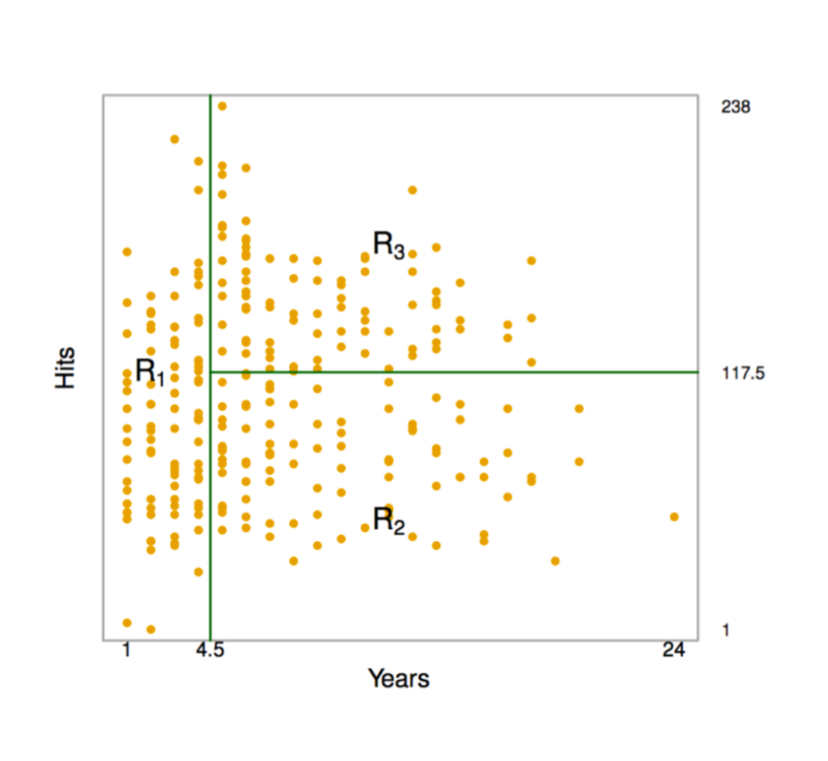
\includegraphics[scale=0.4]{imgs/regression_tree_example2.png}
    \end{center}
\end{column}
\begin{column}{.48\textwidth}
    At each split, we aim to minimize:
    $$\sum_{j=1}^J \sum_{i \in R_j} (y_i - \hat{y}_{R_j})^2$$
\end{column}
\end{columns}
\end{frame}

%%%%%%%%%%%%%%%%%%%%%%%%%%%%%%%%%%%%%%%%%%%%%%%%%%%%%%%%%%%%%%%%%%%%%%%%%%%%%%%

\begin{frame}
\frametitle{Regression Trees: Example}
\begin{table}
\begin{tabular}{c|c|c}
    \hline
    $x_1$   & $x_2$     & $y$ \\
    \hline
    1       & 1         & 1 \\
    0       & 0         & 2 \\
    1       & 0         & 3 \\
    0       & 1         & 4 \\
    \hline
\end{tabular}
\end{table}
\small
Prior to the split we guess the mean, $2.5$, for everything, giving total squared error:

$$E = (1-2.5)^2 + (2-2.5)^2 + (3-2.5)^2 + (4-2.5)^2  = 5$$

After we split on $x_1$ we guess 2 for rows 1 \& 3 and 3 for rows 2 \& 4:

$$ E = (1-2)^2 + (3-2)^2 + (2-3)^2 + (4-3)^2 = 4 $$
\end{frame}

%%%%%%%%%%%%%%%%%%%%%%%%%%%%%%%%%%%%%%%%%%%%%%%%%%%%%%%%%%%%%%%%%%%%%%%%%%%%%%%

\begin{frame}
\frametitle{Decision Tree Summary}
Pros
\begin{itemize}
    \item No feature scaling required
    \item Model nonlinear relationships
    \item Highly interpretable
    \item Can do both classification and regression
    \item Easily deal with continuous or categorical data\textsuperscript{*}
    \item Easily handles missing values\textsuperscript{*}
\end{itemize}

Cons
\begin{itemize}
    \item Can be expensive to train
    \item Often poor predictors - high variance
\end{itemize}

\begin{flushleft}
\tiny{\textsuperscript{*} Not in Python}
\end{flushleft}
\end{frame}

%%%%%%%%%%%%%%%%%%%%%%%%%%%%%%%%%%%%%%%%%%%%%%%%%%%%%%%%%%%%%%%%%%%%%%%%%%%%%%%
\section{Ensemble Methods}
\subsection{}
%%%%%%%%%%%%%%%%%%%%%%%%%%%%%%%%%%%%%%%%%%%%%%%%%%%%%%%%%%%%%%%%%%%%%%%%%%%%%%%

\begin{frame}
\frametitle{Agenda}
\scriptsize
Morning Agenda:

\begin{block}{}
\begin{itemize}
    \item[\checkmark] Review decision trees
    \item Discuss ensemble methods
    \item Discuss \keywd{Bagging} (bootstrap aggregation)
    \item Discuss \keywd{Random Forests}
\end{itemize}
\end{block}

Afternoon Agenda:

\begin{block}{}
\begin{itemize}
    \item Discuss \keywd{Feature Importance}
    \item Discuss \keywd{Out-Of-Bag Error}
\end{itemize}
\end{block}
\end{frame}

%%%%%%%%%%%%%%%%%%%%%%%%%%%%%%%%%%%%%%%%%%%%%%%%%%%%%%%%%%%%%%%%%%%%%%%%%%%%%%%

\begin{frame}
\frametitle{What is an Ensemble Method?}
An \textbf{ensemble model} combines many weak learners to form a strong learner.
\ \\
\ \\
Train multiple different models on the data. To predict:
\begin{itemize}
    \item For regressor, average the predictions of the models
    \item For classifier, take the plurality choice or average the percentages of each class
\end{itemize}
\end{frame}

%%%%%%%%%%%%%%%%%%%%%%%%%%%%%%% %%%%%%%%%%%%%%%%%%%%%%%%%%%%%%%%%%%%%%%%%%%%%%%%

\begin{frame}
\frametitle{Ensembles: Intuition}
Suppose we have 5 \textit{independent} binary classifiers, each 70\% accurate.

Overall accuracy:

$$ \binom{5}{3} 0.7^3 0.3^2 \times \binom{5}{4} 0.7^4 0.3 \times \binom{5}{5} 0.7^5 \approx 0.83 $$

With 101 such classifiers we can achieve 99.9\% accuracy.

\begin{itemize}
    \item Why wouldn't this work?
\end{itemize}
\end{frame}

%%%%%%%%%%%%%%%%%%%%%%%%%%%%%%%%%%%%%%%%%%%%%%%%%%%%%%%%%%%%%%%%%%%%%%%%%%%%%%%

\begin{frame}
\frametitle{Ensembles: Independence}
Unfortunately, if all the learners are the same, creating an ensemble model won't help.
\ \\
\ \\
A solution to this is to train each learner on a different subset of the data.  But how do we do this when we only have one set of data to work with?
\ \\
\ \\
\keywd{Bootstrapping} to the rescue!
\end{frame}

%%%%%%%%%%%%%%%%%%%%%%%%%%%%%%%%%%%%%%%%%%%%%%%%%%%%%%%%%%%%%%%%%%%%%%%%%%%%%%%


%%%%%%%%%%%%%%%%%%%%%%%%%%%%%%%%%%%%%%%%%%%%%%%%%%%%%%%%%%%%%%%%%%%%%%%%%%%%%%%
\section{Bagging}
\subsection{}
%%%%%%%%%%%%%%%%%%%%%%%%%%%%%%%%%%%%%%%%%%%%%%%%%%%%%%%%%%%%%%%%%%%%%%%%%%%%%%%
\begin{frame}
\frametitle{Agenda}
\scriptsize
Morning Agenda:

\begin{block}{}
\begin{itemize}
    \item[\checkmark] Review decision trees
    \item[\checkmark] Discuss ensemble methods
    \item Discuss \keywd{Bagging} (bootstrap aggregation)
    \item Discuss \keywd{Random Forests}
\end{itemize}
\end{block}

Afternoon Agenda:

\begin{block}{}
\begin{itemize}
    \item Discuss \keywd{Feature Importance}
    \item Discuss \keywd{Out-Of-Bag Error}
\end{itemize}
\end{block}
\end{frame}

%%%%%%%%%%%%%%%%%%%%%%%%%%%%%%%%%%%%%%%%%%%%%%%%%%%%%%%%%%%%%%%%%%%%%%%%%%%%%%%

\begin{frame}
\frametitle{Review: Bootstrapping}
Questions:

What is a bootstrap sample?
\visible<2->{
\begin{itemize}
    \item Given $n$ data points we select a sample of $n$ points \textit{with replacement}
\end{itemize}
}

\ \\

What have we learned that bootstrap samples are good for so far?
\visible<3->{
\begin{itemize}
    \item We use bootstrap samples to construct confidence intervals around sample statistics
    \item Ex: If I want a confidence interval around my sample median I could take 1,000 bootstrap samples and take the mean of all 1,000 samples.  These means will follow a normal distribution.
\end{itemize}
}
\end{frame}

%%%%%%%%%%%%%%%%%%%%%%%%%%%%%%%%%%%%%%%%%%%%%%%%%%%%%%%%%%%%%%%%%%%%%%%%%%%%%%%


\begin{frame}
\frametitle{Decision Trees \& Variance}
\footnotesize
\begin{itemize}
    \item Remember that one of the biggest downfalls of using Decision Trees are their inherently large variance, but this is something we can control!
    \item Recall that given a set of $n$ independent observations $Z_1, ..., Z_n$, each with variance $\sigma^2$, the variance of the mean $\bar{Z}$ of the observations is given by $\sigma^2/n$
    \footnotesize
    \begin{itemize}
        \item In other words, \textit{averaging a set of observations reduces variance}
    \end{itemize}
    \item If we would like to reduce the variance of our models predictions (and hence increase the prediction accuracy), we can take many training sets from the population (or \keywd{bootstrap} them!), build separate models for each set, and average the predictions from each
\end{itemize}

\begin{equation}
    \hat{f}_{bag}(x) = \frac{1}{B} \sum_{b=1}^B \hat{f}^{* b}(x)
\end{equation}
\end{frame}

%%%%%%%%%%%%%%%%%%%%%%%%%%%%%%%%%%%%%%%%%%%%%%%%%%%%%%%%%%%%%%%%%%%%%%%%%%%%%%%

\begin{frame}
\frametitle{Bagging = Bootstrap, Fit, Repeat}
\begin{itemize}
    \item \keywd{Bootstrap Aggregation}, or \keywd{bagging}, is a general-purpose procedure for reducing the variance of a statistical learning method
    \item The resulting trees are grown deep and are not pruned.  Hence each individual tree has high variance, but low bias
    \item Averaging these $B$ trees reduces the variance significantly at the cost of a marginal increase in bias
    \item The number of trees $B$ is not a critical parameter with bagging; using a very large $B$ won't lead to overfitting
    \item In practice we want to use a large enough $B$ such that our test error has settled down
\end{itemize}
\end{frame}

%%%%%%%%%%%%%%%%%%%%%%%%%%%%%%%%%%%%%%%%%%%%%%%%%%%%%%%%%%%%%%%%%%%%%%%%%%%%%%%


%%%%%%%%%%%%%%%%%%%%%%%%%%%%%%%%%%%%%%%%%%%%%%%%%%%%%%%%%%%%%%%%%%%%%%%%%%%%%%%
\section{Random Forests}
\subsection{}
%%%%%%%%%%%%%%%%%%%%%%%%%%%%%%%%%%%%%%%%%%%%%%%%%%%%%%%%%%%%%%%%%%%%%%%%%%%%%%%
\begin{frame}
\frametitle{Agenda}
\scriptsize
Morning Agenda:

\begin{block}{}
\begin{itemize}
    \item[\checkmark] Review decision trees
    \item[\checkmark] Discuss ensemble methods
    \item[\checkmark] Discuss \keywd{Bagging} (bootstrap aggregation)
    \item Discuss \keywd{Random Forests}
\end{itemize}
\end{block}

Afternoon Agenda:

\begin{block}{}
\begin{itemize}
    \item Discuss \keywd{Feature Importance}
    \item Discuss \keywd{Out-Of-Bag Error}
\end{itemize}
\end{block}
\end{frame}

%%%%%%%%%%%%%%%%%%%%%%%%%%%%%%%%%%%%%%%%%%%%%%%%%%%%%%%%%%%%%%%%%%%%%%%%%%%%%%%

\begin{frame}
\frametitle{Random Forests}
\begin{itemize}
    \item \keywd{Random Forests} provide an improvement over bagged trees by the way of a small tweak that serves to \keywd{decorrelate} the trees
    \item At each split in a given tree, a \textit{random sample of $m$ predictors} are chosen as candidates from the full set of $p$ predictors.
    \begin{itemize}
        \item Often $m = \sqrt{p}$
    \end{itemize}
    \item This technique, called \textbf{subset sampling}, serves to prevent trees from always choosing the same splits
    \item As with bagging, random forests will not overfit if we increase $B$, so in practice we use a value of $B$ sufficiently large for the error rate to have settled down
\end{itemize}
\end{frame}

%%%%%%%%%%%%%%%%%%%%%%%%%%%%%%%%%%%%%%%%%%%%%%%%%%%%%%%%%%%%%%%%%%%%%%%%%%%%%%%

\begin{frame}
\frametitle{Random Forest Parameters}
Random Forest Parameters:
\begin{itemize}
    \item Total number of trees (\mintinline{python}{n_estimators})
    \item Number of features to use at each split (\mintinline{python}{max_features})
    \item Number of points for each bootstrap sample
    \item Individual decision tree parameters
    \begin{itemize}
        \item e.g. tree depth, pruning (\mintinline{python}{min_samples_split}, \mintinline{python}{min_samples_leaf}, \& c.)
    \end{itemize}
\end{itemize}

In general, Random Forests are fairly robust to the choice of parameters and overfitting

\end{frame}

%%%%%%%%%%%%%%%%%%%%%%%%%%%%%%%%%%%%%%%%%%%%%%%%%%%%%%%%%%%%%%%%%%%%%%%%%%%%%%%

\begin{frame}
\frametitle{Pros and Cons of Random Forests}
Pros:
\begin{itemize}
    \item Often give near state-of-the-art performance
    \item Good out-of-the-box performance
    \item No feature scaling needed
    \item Model nonlinear relationships
\end{itemize}

Cons:
\begin{itemize}
    \item Can be expensive to train (though can be done in parallel)
    \item Models can be quite large (the pickled version of a several hundred tree model can easily be several GBs)
    \item Not interpretable (although techniques such as predicted value plots can help)
\end{itemize}
\end{frame}

%%%%%%%%%%%%%%%%%%%%%%%%%%%%%%%%%%%%%%%%%%%%%%%%%%%%%%%%%%%%%%%%%%%%%%%%%%%%%%%

\begin{frame}[fragile]{}
\frametitle{Random Forests in Scikit-Learn}
\scriptsize
The following is an example of how one can implement a Random Forest using scikit-learn:

\begin{minted}[linenos, gobble=4, fontsize=\scriptsize]{python}
    from sklearn.ensemble import RandomForestRegressor
    from sklearn.metrics import mean_squared_error
    from sklearn.cross_validation import train_test_split

    y = df.pop('target').values
    X = df.values
    X_train, X_test, y_train, y_test = train_test_split(X, y, test_size=0.33, \
                                                        random_state=42)

    rf = RandomForestRegressor(n_estimators=100)
    rf.fit(X_train, y_train)
    y_pred = rf.predict(X_test)
    print(mean_squared_error(y_test, y_pred))
\end{minted}
\end{frame}

%%%%%%%%%%%%%%%%%%%%%%%%%%%%%%%%%%%%%%%%%%%%%%%%%%%%%%%%%%%%%%%%%%%%%%%%%%%%%

\begin{frame}
\frametitle{Objectives}
\scriptsize

Morning Objectives:
\begin{block}{}
\begin{itemize}
    \item[\checkmark] Review of Decision Trees
    \visible<2->{
    \item[\checkmark] Explain the relationship and difference between \keywd{bagging} and random forests
    }
    \visible<3->{
    \item[\checkmark] Explain the construction of a \keywd{Random Forest} (classification or regression) algorithm
    }
    \visible<4->{
    \item[\checkmark] Explain why random forests often perform better than a single decision tree
    }
\end{itemize}
\end{block}
\end{frame}

%%%%%%%%%%%%%%%%%%%%%%%%%%%%%%%%%%%%%%%%%%%%%%%%%%%%%%%%%%%%%%%%%%%%%%%%%%%%%%%

%%%%%%%%%%%%%%%%%%%%%%%%%%%%%%%%%%%%%%%%%%%%%%%%%%%%%%%%%%%%%%%%%%%%%%%%%%%%%%%
\section{Feature Importances}
\subsection{}
%%%%%%%%%%%%%%%%%%%%%%%%%%%%%%%%%%%%%%%%%%%%%%%%%%%%%%%%%%%%%%%%%%%%%%%%%%%%%%%

\begin{frame}
\frametitle{Agenda}
\scriptsize
Morning Agenda:

\begin{block}{}
\begin{itemize}
    \item[\checkmark] Review decision trees
    \item[\checkmark] Discuss ensemble methods
    \item[\checkmark] Discuss \keywd{Bagging} (bootstrap aggregation)
    \item[\checkmark] Discuss \keywd{Random Forests}
\end{itemize}
\end{block}

Afternoon Agenda:

\begin{block}{}
\begin{itemize}
    \item Discuss \keywd{Feature Importance}
    \item Discuss \keywd{Out-Of-Bag Error}
\end{itemize}
\end{block}
\end{frame}

%%%%%%%%%%%%%%%%%%%%%%%%%%%%%%%%%%%%%%%%%%%%%%%%%%%%%%%%%%%%%%%%%%%%%%%%%%%%%%%

\begin{frame}
\frametitle{Measuring Feature Importance}
\begin{itemize}
    \item When we bag a large number of trees, it is no longer possible to represent the resulting statistical learning procedure using a single tree and it is difficult to ascertain which features are most important
    \item There are several ways we can go about attempting to identify the most important features including:
    \begin{itemize}
        \item Measuring the total amount that the RSS is decreased due to splits over a given predictor (regression trees).
        \item Record what proportion of points pass through a split; the higher in the tree a feature is, the more important.  Average this proportion across all trees.
        \item When the $B_i$ tree is grown, pass OOB through it.  Permute or remove feature $X_j$ and measure the change in accuracy (or other metric) before and after permuting/removing
    \end{itemize}
\end{itemize}
\end{frame}

%%%%%%%%%%%%%%%%%%%%%%%%%%%%%%%%%%%%%%%%%%%%%%%%%%%%%%%%%%%%%%%%%%%%%%%%%%%%%%%

\begin{frame}
\frametitle{Feature Importance in Scikit-Learn}
When training a random forest model in Scikit-Learn there is an attribute called \mintinline{python}{model.feature_importances_} which stores normalized importances for each of our models features

\begin{itemize}
    \item \"It is sometimes called \'gini importance' or \'mean decrease impurity' and is defined as the total decrease in node impurity (weighted by the probability of reaching that node) averaged over all trees of the ensemble."
\end{itemize}
\end{frame}

%%%%%%%%%%%%%%%%%%%%%%%%%%%%%%%%%%%%%%%%%%%%%%%%%%%%%%%%%%%%%%%%%%%%%%%%%%%%%%%

\begin{frame}
\frametitle{Computing Feature Importance On Single Tree}
For some intuition, this is how this is calculated on a tree by tree basis and then averaged across all the trees in our model

\begin{enumerate}
    \item Initialize array \mintinline{python}{feature_importances} of all zeros with size \mintinline{python}{n_features}
    \item Traverse the tree
    \begin{itemize}
        \item For each internal node that splits on feature \mintinline{python}{i}, compute the error reduction of that node multiplied by the number of samples that were routed to the node
        \item Add this quantity to \mintinline{python}{feature_importances[i]}
    \end{itemize}
\end{enumerate}

The error reduction depends on the impurity criterion that you use (e.g. Gini, Entroy, RSS).  The result is, by default, normalized in sklearn.

\end{frame}

%%%%%%%%%%%%%%%%%%%%%%%%%%%%%%%%%%%%%%%%%%%%%%%%%%%%%%%%%%%%%%%%%%%%%%%%%%%%%%%

\begin{frame}
\frametitle{Example Feature Importance Plot}
\begin{center}
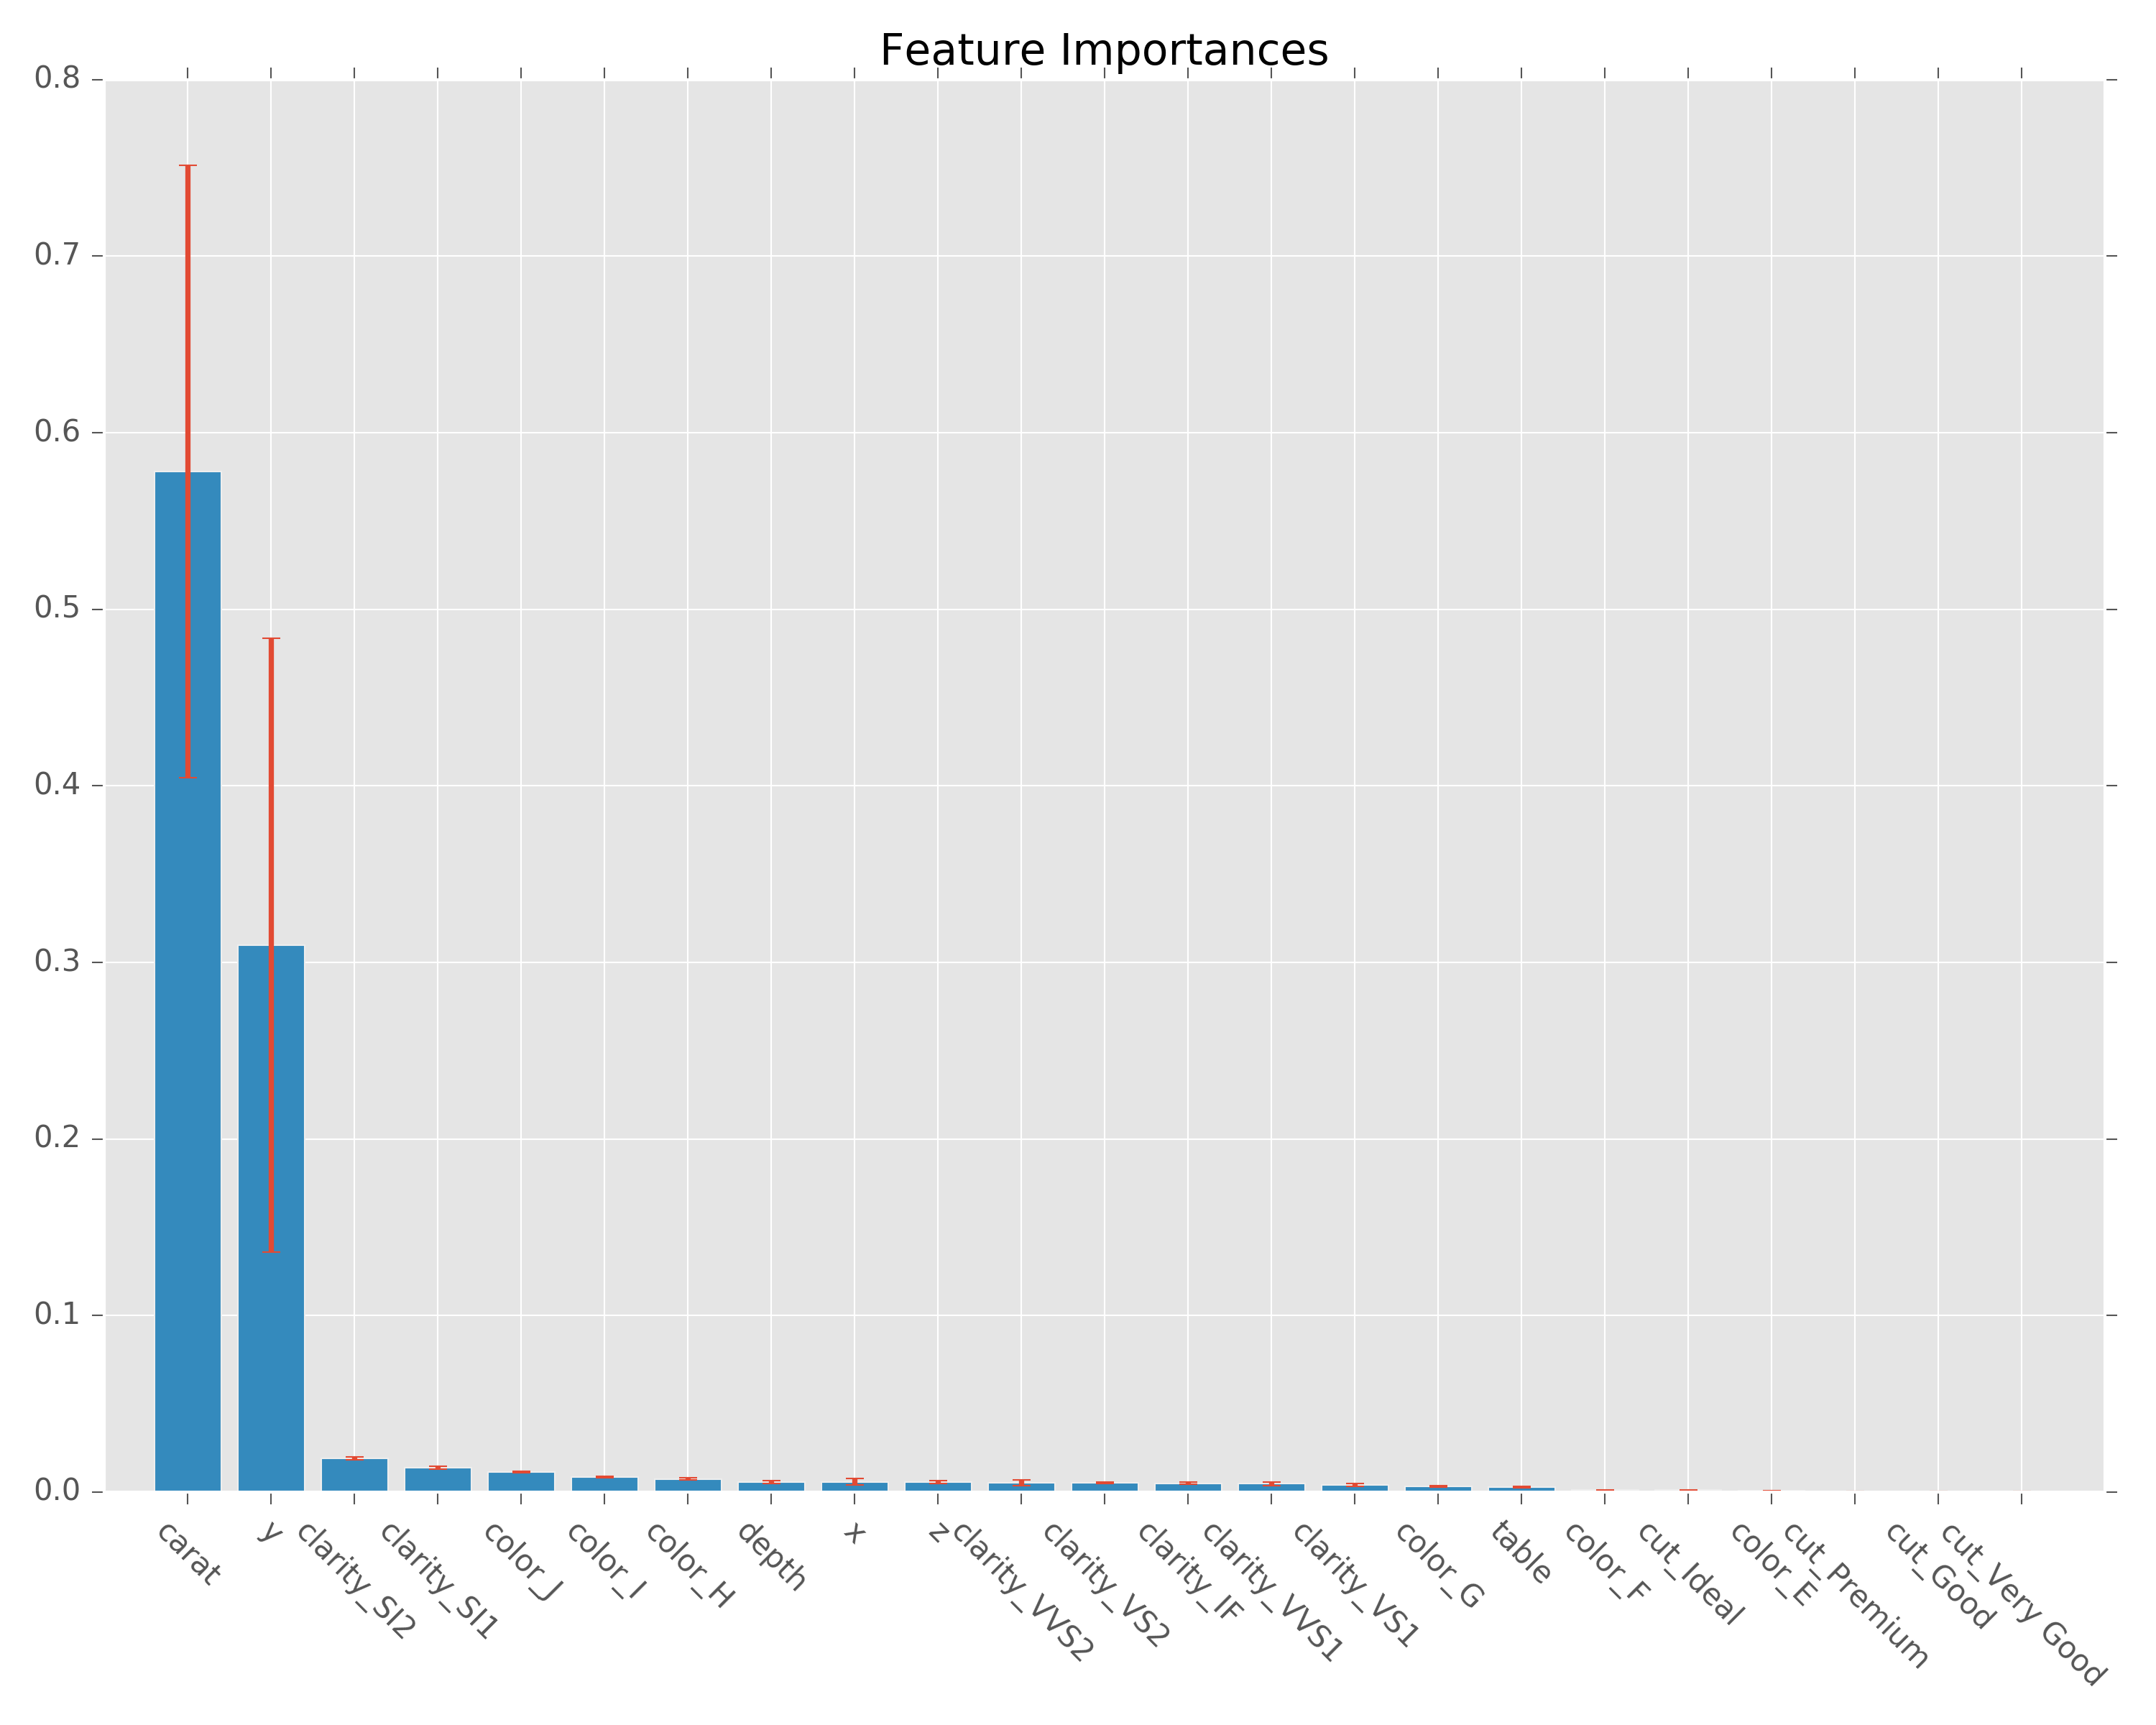
\includegraphics[scale=0.35]{imgs/sklearn_feature_importance.png}
\end{center}
\end{frame}

%%%%%%%%%%%%%%%%%%%%%%%%%%%%%%%%%%%%%%%%%%%%%%%%%%%%%%%%%%%%%%%%%%%%%%%%%%%%%%%

\begin{frame}
\frametitle{Leave One Out Feature Importance}
There are, of course, other ways we might choose to measure how important a feature is.

\begin{itemize}
    \item One way is to iteratively drop each feature, train a new model, and compare the MSE before and after (in the regression case)
    \item A feature which wasn't important will have a low effect on the model before and after removal
\end{itemize}
\end{frame}

%%%%%%%%%%%%%%%%%%%%%%%%%%%%%%%%%%%%%%%%%%%%%%%%%%%%%%%%%%%%%%%%%%%%%%%%%%%%%%%

\begin{frame}
\frametitle{Leave One Out Feature Importance}
\begin{center}
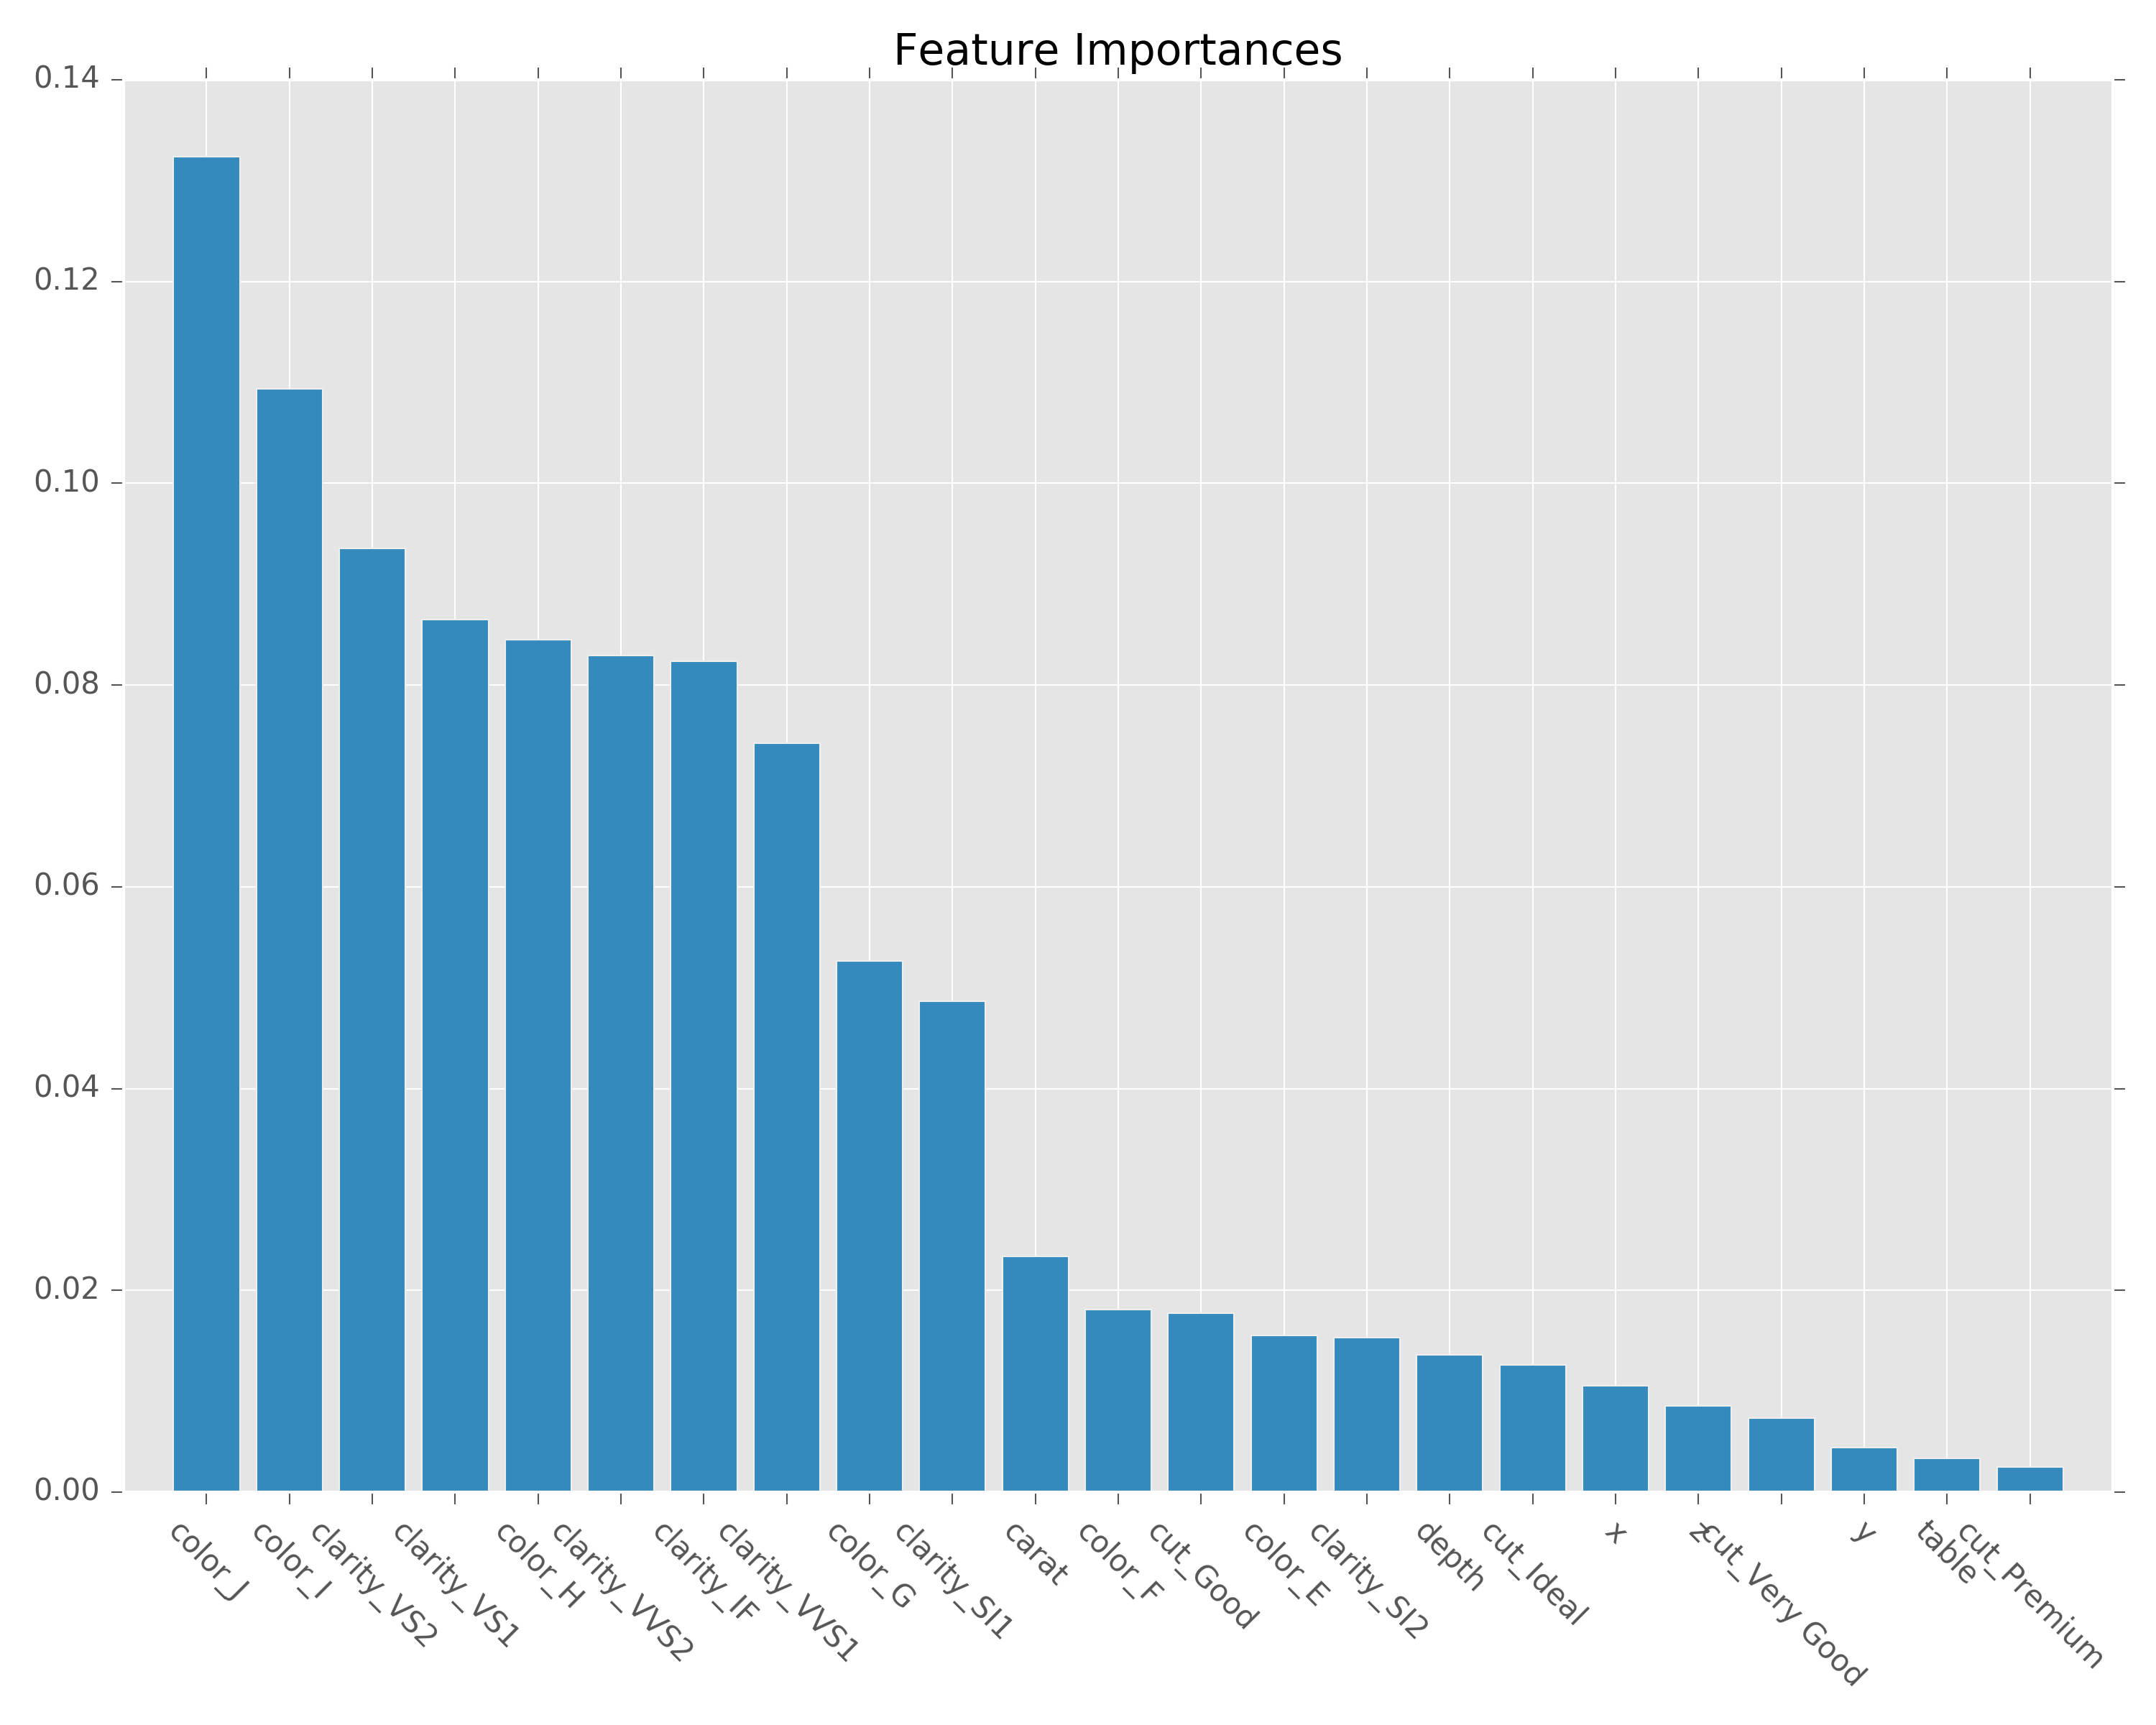
\includegraphics[scale=0.35]{imgs/loo_feature_importance.png}
\end{center}
\end{frame}

%%%%%%%%%%%%%%%%%%%%%%%%%%%%%%%%%%%%%%%%%%%%%%%%%%%%%%%%%%%%%%%%%%%%%%%%%%%%%%%

\begin{frame}
\frametitle{Stop and Think}
Why do you think these measures of importance were so different?

\begin{itemize}
    \visible<2->{
    \item One possible explaination is that features that were deemed to be important in our initial feature importance plot can be represented by other features in our dataset.  For example, \mintinline{python}{carat} (a measure of weight) can likely be accurately represented by \mintinline{python}{x}, \mintinline{python}{y}, \mintinline{python}{z} (length, width, and depth respectively)
    }
    \visible<3->{
    \item This also points out a crucial nuance to Scikit-Learn's measure of feature importance: continuous features and categorical variables with many levels are often deemed more important than categorical variables with fewer levels
    }
\end{itemize}
\end{frame}

%%%%%%%%%%%%%%%%%%%%%%%%%%%%%%%%%%%%%%%%%%%%%%%%%%%%%%%%%%%%%%%%%%%%%%%%%%%%%%%
\section{Out-Of-Bag Error}
\subsection{}
%%%%%%%%%%%%%%%%%%%%%%%%%%%%%%%%%%%%%%%%%%%%%%%%%%%%%%%%%%%%%%%%%%%%%%%%%%%%%%%

\begin{frame}
\frametitle{Agenda}
\scriptsize
Morning Agenda:

\begin{block}{}
\begin{itemize}
    \item[\checkmark] Review decision trees
    \item[\checkmark] Discuss ensemble methods
    \item[\checkmark] Discuss \keywd{Bagging} (bootstrap aggregation)
    \item[\checkmark] Discuss \keywd{Random Forests}
\end{itemize}
\end{block}

Afternoon Agenda:

\begin{block}{}
\begin{itemize}
    \item[\checkmark] Discuss \keywd{Feature Importance}
    \item Discuss \keywd{Out-Of-Bag Error}
\end{itemize}
\end{block}
\end{frame}

%%%%%%%%%%%%%%%%%%%%%%%%%%%%%%%%%%%%%%%%%%%%%%%%%%%%%%%%%%%%%%%%%%%%%%%%%%%%%%%

\begin{frame}[fragile]{}
\frametitle{Out-Of-Bag Error Estimation}
\begin{itemize}
    \item One nice side effect from using bootstrapped models is we can easily estimate the test error of a bagged model without the need to perform cross-validation!
    \item Each tree in our forest has only seen ~66\% of our training data
    \item We can thus measure the test error of a particular tree by running the remaining \textit{out-of-bag} (\keywd{OOB})observations through the tree
\end{itemize}

\begin{minted}[linenos, gobble=4, fontsize=\scriptsize]{python}
    rf = RandomForestRegressor(n_estimators=20, oob_score=True)
    rf.fit(X, y)

    print rf.oob_score_
\end{minted}
\end{frame}

%%%%%%%%%%%%%%%%%%%%%%%%%%%%%%%%%%%%%%%%%%%%%%%%%%%%%%%%%%%%%%%%%%%%%%%%%%%%%%%

\begin{frame}
\frametitle{Objectives}
\scriptsize

Afternoon Objectives:
\begin{block}{}
\begin{itemize}
    \item[\checkmark] Explain how to get \keywd{feature importances} from a random forest and what those importances mean
    \visible<2->{
    \item[\checkmark] Explain \keywd{OOB error} is calculated and what it is an estimate of
    }
\end{itemize}
\end{block}

\end{frame}

%%%%%%%%%%%%%%%%%%%%%%%%%%%%%%%%%%%%%%%%%%%%%%%%%%%%%%%%%%%%%%%%%%%%%%%%%%%%%%%




\end{document}
